\hypertarget{a00003}{
\section{Dokumentacja klasy ASS8.Klient.Form1}
\label{d1/d7c/a00003}\index{ASS8::Klient::Form1@{ASS8::Klient::Form1}}
}
Klasa odpowiedzialna za wyświetlenie okna z wyszukiwaniem plików znajomych.  


Diagram współpracy dla ASS8.Klient.Form1:\nopagebreak
\begin{figure}[H]
\begin{center}
\leavevmode
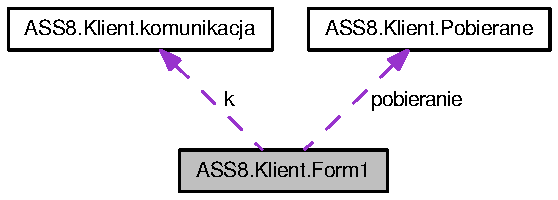
\includegraphics[width=304pt]{dc/d9a/a00218}
\end{center}
\end{figure}
\subsection*{Metody publiczne}
\begin{CompactItemize}
\item 
\hyperlink{a00003_f4f57fa006228bda67e1478113bbd3bd}{Form1} ()
\begin{CompactList}\small\item\em Konstruktor klasy. \item\end{CompactList}\end{CompactItemize}
\subsection*{Atrybuty publiczne}
\begin{CompactItemize}
\item 
\hyperlink{a00013}{komunikacja} \hyperlink{a00003_3a7a9649738431ac4b2dd14fdabb7d1c}{k}
\end{CompactItemize}
\subsection*{Metody prywatne}
\begin{CompactItemize}
\item 
void \hyperlink{a00003_e934f222567288447b30be318da95ba7}{btnListuj\_\-Click} (object sender, EventArgs e)
\begin{CompactList}\small\item\em Funkcja odpowiedzialna za listowanie plików wpisanego użytkownika. \item\end{CompactList}\item 
void \hyperlink{a00003_3565ea2384b6428312fa310aad4c7e25}{button1\_\-Click} (object sender, EventArgs e)
\begin{CompactList}\small\item\em Funkcja odpowiedzialna za obslugę przycisku pobierającego zaznaczone pliku. \item\end{CompactList}\item 
void \hyperlink{a00003_21b906fd66030071dd1057fe32efeca1}{pobieraj} (object o)
\begin{CompactList}\small\item\em Funkcja pobierająca wybrane \hyperlink{a00017}{pliki} z serwera. \item\end{CompactList}\item 
void \hyperlink{a00003_1fb4fa2454ffdf753cce1637657029c8}{btnPobierane\_\-Click} (object sender, EventArgs e)
\begin{CompactList}\small\item\em Przycisk wyswietla pobierane aktualnie \hyperlink{a00017}{pliki} (i zakonczone). \item\end{CompactList}\item 
void \hyperlink{a00003_657650d2f810f254f265eb4956810386}{button2\_\-Click} (object sender, EventArgs e)
\begin{CompactList}\small\item\em Funkcja zamyka okno. \item\end{CompactList}\item 
void \hyperlink{a00003_8f11bfa541be459982c72ad615898de7}{lvPliki\_\-SelectedIndexChanged} (object sender, EventArgs e)
\end{CompactItemize}
\subsection*{Atrybuty prywatne}
\begin{CompactItemize}
\item 
\hyperlink{a00019}{Pobierane} \hyperlink{a00003_a21006ffcd0ae9b655d6232326c0783e}{pobieranie} = null
\item 
string \hyperlink{a00003_8647bc097f5550069c2ffa260182726e}{wyswietlonePliki}
\item 
Mutex \hyperlink{a00003_26249d134376a8c1b9be63c9a2df68a2}{mut} = new Mutex()
\end{CompactItemize}


\subsection{Opis szczegółowy}
Klasa odpowiedzialna za wyświetlenie okna z wyszukiwaniem plików znajomych. 



Definicja w linii 16 pliku Znajomi.cs.

\subsection{Dokumentacja konstruktora i destruktora}
\hypertarget{a00003_f4f57fa006228bda67e1478113bbd3bd}{
\index{ASS8::Klient::Form1@{ASS8::Klient::Form1}!Form1@{Form1}}
\index{Form1@{Form1}!ASS8::Klient::Form1@{ASS8::Klient::Form1}}
\subsubsection[{Form1}]{\setlength{\rightskip}{0pt plus 5cm}ASS8.Klient.Form1.Form1 ()}}
\label{d1/d7c/a00003_f4f57fa006228bda67e1478113bbd3bd}


Konstruktor klasy. 



Definicja w linii 23 pliku Znajomi.cs.

\subsection{Dokumentacja funkcji składowych}
\hypertarget{a00003_e934f222567288447b30be318da95ba7}{
\index{ASS8::Klient::Form1@{ASS8::Klient::Form1}!btnListuj\_\-Click@{btnListuj\_\-Click}}
\index{btnListuj\_\-Click@{btnListuj\_\-Click}!ASS8::Klient::Form1@{ASS8::Klient::Form1}}
\subsubsection[{btnListuj\_\-Click}]{\setlength{\rightskip}{0pt plus 5cm}void ASS8.Klient.Form1.btnListuj\_\-Click (object {\em sender}, \/  EventArgs {\em e})\hspace{0.3cm}{\tt  \mbox{[}private\mbox{]}}}}
\label{d1/d7c/a00003_e934f222567288447b30be318da95ba7}


Funkcja odpowiedzialna za listowanie plików wpisanego użytkownika. 

\begin{Desc}
\item[Parametry:]
\begin{description}
\item[{\em sender}]\item[{\em e}]\end{description}
\end{Desc}


Definicja w linii 40 pliku Znajomi.cs.

Oto graf wywołań dla tej funkcji:\nopagebreak
\begin{figure}[H]
\begin{center}
\leavevmode
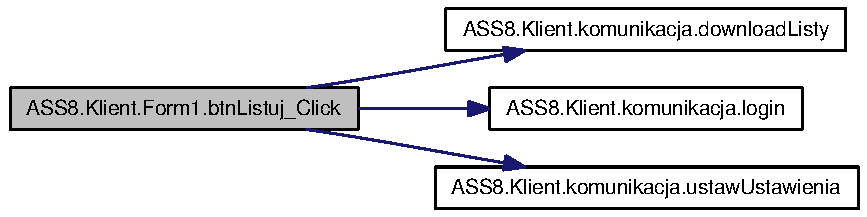
\includegraphics[width=226pt]{d1/d7c/a00003_e934f222567288447b30be318da95ba7_cgraph}
\end{center}
\end{figure}
\hypertarget{a00003_1fb4fa2454ffdf753cce1637657029c8}{
\index{ASS8::Klient::Form1@{ASS8::Klient::Form1}!btnPobierane\_\-Click@{btnPobierane\_\-Click}}
\index{btnPobierane\_\-Click@{btnPobierane\_\-Click}!ASS8::Klient::Form1@{ASS8::Klient::Form1}}
\subsubsection[{btnPobierane\_\-Click}]{\setlength{\rightskip}{0pt plus 5cm}void ASS8.Klient.Form1.btnPobierane\_\-Click (object {\em sender}, \/  EventArgs {\em e})\hspace{0.3cm}{\tt  \mbox{[}private\mbox{]}}}}
\label{d1/d7c/a00003_1fb4fa2454ffdf753cce1637657029c8}


Przycisk wyswietla pobierane aktualnie \hyperlink{a00017}{pliki} (i zakonczone). 

\begin{Desc}
\item[Parametry:]
\begin{description}
\item[{\em sender}]\item[{\em e}]\end{description}
\end{Desc}


Definicja w linii 114 pliku Znajomi.cs.\hypertarget{a00003_3565ea2384b6428312fa310aad4c7e25}{
\index{ASS8::Klient::Form1@{ASS8::Klient::Form1}!button1\_\-Click@{button1\_\-Click}}
\index{button1\_\-Click@{button1\_\-Click}!ASS8::Klient::Form1@{ASS8::Klient::Form1}}
\subsubsection[{button1\_\-Click}]{\setlength{\rightskip}{0pt plus 5cm}void ASS8.Klient.Form1.button1\_\-Click (object {\em sender}, \/  EventArgs {\em e})\hspace{0.3cm}{\tt  \mbox{[}private\mbox{]}}}}
\label{d1/d7c/a00003_3565ea2384b6428312fa310aad4c7e25}


Funkcja odpowiedzialna za obslugę przycisku pobierającego zaznaczone pliku. 

\begin{Desc}
\item[Parametry:]
\begin{description}
\item[{\em sender}]\item[{\em e}]\end{description}
\end{Desc}


Definicja w linii 69 pliku Znajomi.cs.\hypertarget{a00003_657650d2f810f254f265eb4956810386}{
\index{ASS8::Klient::Form1@{ASS8::Klient::Form1}!button2\_\-Click@{button2\_\-Click}}
\index{button2\_\-Click@{button2\_\-Click}!ASS8::Klient::Form1@{ASS8::Klient::Form1}}
\subsubsection[{button2\_\-Click}]{\setlength{\rightskip}{0pt plus 5cm}void ASS8.Klient.Form1.button2\_\-Click (object {\em sender}, \/  EventArgs {\em e})\hspace{0.3cm}{\tt  \mbox{[}private\mbox{]}}}}
\label{d1/d7c/a00003_657650d2f810f254f265eb4956810386}


Funkcja zamyka okno. 

\begin{Desc}
\item[Parametry:]
\begin{description}
\item[{\em sender}]\item[{\em e}]\end{description}
\end{Desc}


Definicja w linii 130 pliku Znajomi.cs.\hypertarget{a00003_8f11bfa541be459982c72ad615898de7}{
\index{ASS8::Klient::Form1@{ASS8::Klient::Form1}!lvPliki\_\-SelectedIndexChanged@{lvPliki\_\-SelectedIndexChanged}}
\index{lvPliki\_\-SelectedIndexChanged@{lvPliki\_\-SelectedIndexChanged}!ASS8::Klient::Form1@{ASS8::Klient::Form1}}
\subsubsection[{lvPliki\_\-SelectedIndexChanged}]{\setlength{\rightskip}{0pt plus 5cm}void ASS8.Klient.Form1.lvPliki\_\-SelectedIndexChanged (object {\em sender}, \/  EventArgs {\em e})\hspace{0.3cm}{\tt  \mbox{[}private\mbox{]}}}}
\label{d1/d7c/a00003_8f11bfa541be459982c72ad615898de7}




Definicja w linii 135 pliku Znajomi.cs.\hypertarget{a00003_21b906fd66030071dd1057fe32efeca1}{
\index{ASS8::Klient::Form1@{ASS8::Klient::Form1}!pobieraj@{pobieraj}}
\index{pobieraj@{pobieraj}!ASS8::Klient::Form1@{ASS8::Klient::Form1}}
\subsubsection[{pobieraj}]{\setlength{\rightskip}{0pt plus 5cm}void ASS8.Klient.Form1.pobieraj (object {\em o})\hspace{0.3cm}{\tt  \mbox{[}private\mbox{]}}}}
\label{d1/d7c/a00003_21b906fd66030071dd1057fe32efeca1}


Funkcja pobierająca wybrane \hyperlink{a00017}{pliki} z serwera. 

\begin{Desc}
\item[Parametry:]
\begin{description}
\item[{\em o}]\end{description}
\end{Desc}


Definicja w linii 91 pliku Znajomi.cs.

\subsection{Dokumentacja atrybutów składowych}
\hypertarget{a00003_3a7a9649738431ac4b2dd14fdabb7d1c}{
\index{ASS8::Klient::Form1@{ASS8::Klient::Form1}!k@{k}}
\index{k@{k}!ASS8::Klient::Form1@{ASS8::Klient::Form1}}
\subsubsection[{k}]{\setlength{\rightskip}{0pt plus 5cm}{\bf komunikacja} {\bf ASS8.Klient.Form1.k}}}
\label{d1/d7c/a00003_3a7a9649738431ac4b2dd14fdabb7d1c}




Definicja w linii 19 pliku Znajomi.cs.\hypertarget{a00003_26249d134376a8c1b9be63c9a2df68a2}{
\index{ASS8::Klient::Form1@{ASS8::Klient::Form1}!mut@{mut}}
\index{mut@{mut}!ASS8::Klient::Form1@{ASS8::Klient::Form1}}
\subsubsection[{mut}]{\setlength{\rightskip}{0pt plus 5cm}Mutex {\bf ASS8.Klient.Form1.mut} = new Mutex()\hspace{0.3cm}{\tt  \mbox{[}private\mbox{]}}}}
\label{d1/d7c/a00003_26249d134376a8c1b9be63c9a2df68a2}




Definicja w linii 86 pliku Znajomi.cs.\hypertarget{a00003_a21006ffcd0ae9b655d6232326c0783e}{
\index{ASS8::Klient::Form1@{ASS8::Klient::Form1}!pobieranie@{pobieranie}}
\index{pobieranie@{pobieranie}!ASS8::Klient::Form1@{ASS8::Klient::Form1}}
\subsubsection[{pobieranie}]{\setlength{\rightskip}{0pt plus 5cm}{\bf Pobierane} {\bf ASS8.Klient.Form1.pobieranie} = null\hspace{0.3cm}{\tt  \mbox{[}private\mbox{]}}}}
\label{d1/d7c/a00003_a21006ffcd0ae9b655d6232326c0783e}




Definicja w linii 18 pliku Znajomi.cs.\hypertarget{a00003_8647bc097f5550069c2ffa260182726e}{
\index{ASS8::Klient::Form1@{ASS8::Klient::Form1}!wyswietlonePliki@{wyswietlonePliki}}
\index{wyswietlonePliki@{wyswietlonePliki}!ASS8::Klient::Form1@{ASS8::Klient::Form1}}
\subsubsection[{wyswietlonePliki}]{\setlength{\rightskip}{0pt plus 5cm}string {\bf ASS8.Klient.Form1.wyswietlonePliki}\hspace{0.3cm}{\tt  \mbox{[}private\mbox{]}}}}
\label{d1/d7c/a00003_8647bc097f5550069c2ffa260182726e}




Definicja w linii 34 pliku Znajomi.cs.

Dokumentacja dla tej klasy została wygenerowana z pliku:\begin{CompactItemize}
\item 
\hyperlink{a00057}{Znajomi.cs}\end{CompactItemize}
